% !TEX root=report.tex
\section{Problem Formalization and Prediction Model} \label{sec:model}

Now we formalize the problem and present our model.
All notation is also presented in \autoref{tab:notation} for reference.

\begin{table}
\centering
\caption{Summary of our notation.}
\label{tab:notation}
\begin{tabular}{lp{7cm}}
Symbol & Meaning\\
\hline
$h \in \mathcal{H}$   & Host, from a set of all users who have received at least $K$ couch requests. \\ 
$\mathcal{S}_h$       & Set of all competitor sets $S$ for host $h$. \\
$S \in \mathcal{S}_h$ & Competitor set for host $h$, composed of surfers who have made a couch request to $h$ at roughly the same time. \\
$\Phi(s,h,c)$         & Featurization function mapping a couch request from a surfer to a host to $\mathbb{R}^D.$\\
$\theta$,$r$          & Global parameters: weights for the couch request features, and a ``reject-all'' parameter.\\
$\theta_h$,$r_h$      & Corresponding host-specific parameters.\\
\hline
\end{tabular}\end{table}

From the CouchSurfing user database, we form a set of \emph{hosts} $\mathcal{H}$ such that every $h \in \mathcal{H}$ has hosted at least $K$ persons since signing up for a user account.
We initially set $K=1$; a higher setting may reduce the amount of noise in the set of hosts.

For every host $h$, there is at least one \emph{competitor set} $S$ of at least $K$ \emph{surfers}, where each surfer $s \in S$ has made a couch request to $h$.
A competitor set corresponds to a decision made by the host to either host one of the $s$ in the set, or to reject all of them.
The composition of this set is inferred from data based on the timing of couch requests and host decisions.
This is discussed in \autoref{subsec:competitor_sets}.

In fact, $h$ may have multiple such competitor sets.
We refer to the set of competitor sets for host $h$ by $\mathcal{S}_h$.

% !TEX root=report.tex
\subsection{Competitor Sets} \label{subsec:competitor_sets}

The data we received from CouchSurfing does not allow us to know exactly when a host has looked at a couch request, but it does have timestamps for every request and every decision made by a host.
To form sets of ``competing'' requests, we use a heuristic procedure to scan through all requests made to a particular host, and split them into groups based on their timing, their requested lodging dates, and the timing of the host's decisions.

In the following, requests carry the same index as the user/surfer that invoked them, i.e., surfer $s_i$ sends request $c_{i,j}$ to host $h_j$.
Without loss of generality we can assume for now that each user just sends at most one request to each couch.
In the following examples, $h$ is fixed, so we just denote requests as $c_i$.
 
The CS system allows hosts to reject a couch request, which indicates a negative sample. We call those \textit{explicit negatives}. In addition, it is possible to infer \textit{implicit negatives}: if we take for example a host $h$ with a very popular couch in Paris with tens of requests per day, it seems reasonable to assume that $h$ will not look at every request, and will stop reading more requests after deciding for a specific surfer $s_i$.
These requests won't receive an explicit Reject, but are \emph{de facto} rejected due to ``timing out.''

For a given period $\tau$, let $C_{j}^{\tau} = c_1, c_2,\ldots,c_n$ be the requests send to $h$. We hereby assume that if at a certain time host $h$ accepts a request $c_i$ for period $\tau$, she prefers the requesting surfer $s_i$ over all other users whose requests she read that overlap with $\tau$. An efficient sweep-line algorithm to find sets of overlapping requests is depicted in {algorithm~\ref{alg:overlap}}.

One more important thing to keep in mind is that if $h$ accepted a request for period $\tau$ at time $t_0$ and gets another request $c_l$ for $\tau$ at time $t_1 > t_0$, there is no information about whether or not $h$ likes $s_i$, because his couch is already taken, so we have to filter these out before moving on.

\begin{algorithm}
\caption{Find overlapping requests}
\label{alg:overlap}
\begin{algorithmic} 
\REQUIRE $R = (c_1, c_2,\ldots,c_n)$, $c_i = (t_i^{start}, t_i^{end})$
\ENSURE $S\subseteq \mathcal{P}(R)$ 
\STATE $S \leftarrow \emptyset$
\STATE $A \leftarrow \emptyset$ 
\STATE $T {(i, start/end, t_i^{s/t}) |c_i \in R}$
\STATE $sort(T, t_i^{s/t})$ 
\STATE $b\_incr \leftarrow True$ 
\FOR{$t$ in $T$}
\IF{$t$ == $v_j^{start}$}
\STATE $A.append(t)$
\STATE $b\_incr \leftarrow True$
\ELSE
\IF{$b\_incr == True$}
\STATE $b\_incr \leftarrow False$
\STATE $S.append({c_i | (i, \_, \_) \in A})$
\ENDIF
\STATE $A.delete(t)$
\ENDIF
\ENDFOR
\end{algorithmic}
\end{algorithm}

It might also be beneficial to soften the notion of ``overlap'' just because it might be very stressful for a host to have surfers without a gap in between the two visits.

Analyzing the data for statistics on gaps for each host seperately will reveal their willingness to host several surfers in a row.
The above algorithm can easily be adapted by modifying the input times accordingly.
\todo{for tobi: clarify this: is this used?}

\subsubsection{Filter rejects by temporal constraints}
\todo{for tobi: i'm confused---how is what was done above different from this? maybe unite?}

\todo{for tobi: insert reference to \autoref{fig:timeline_view} somewhere.}

Using a very similar technique we can filter rejects that are not actually rejects for the reason of a mismatching surfer. Imagine $h$ gets a request $c_1$ at time $t_1$, accepts this request at time $t_2$ and gets another request $c_2$ for the same period as $c_1$ at $t_3$. If we have that $t_1 < t_2 < t_3$, there is no valid information about whether or not $h$ likes surfer $s_2$. By the time he gets the second request, his couch is already booked out and so he has to reject $s_2$ no matter if he would even prefer him over $s_1$. Because of this scenario we filter our training data for exactly those \textit{uninformative rejects} using again algorithm~\ref{alg:overlap} and temporal orderings on requests and acceptances/rejects.

\begin{figure}[ht]
\centering
\subfloat[Requested]{
  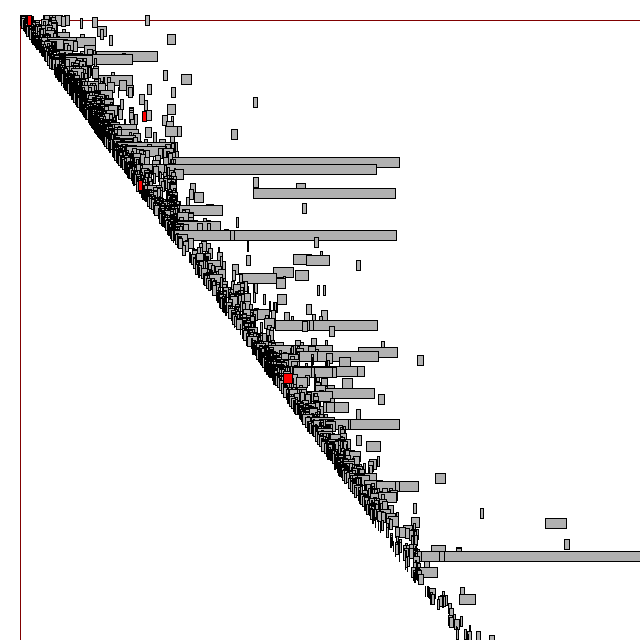
\includegraphics[width=0.45\linewidth]{figures/top_requested.png}
}
\subfloat[Accepted]{
  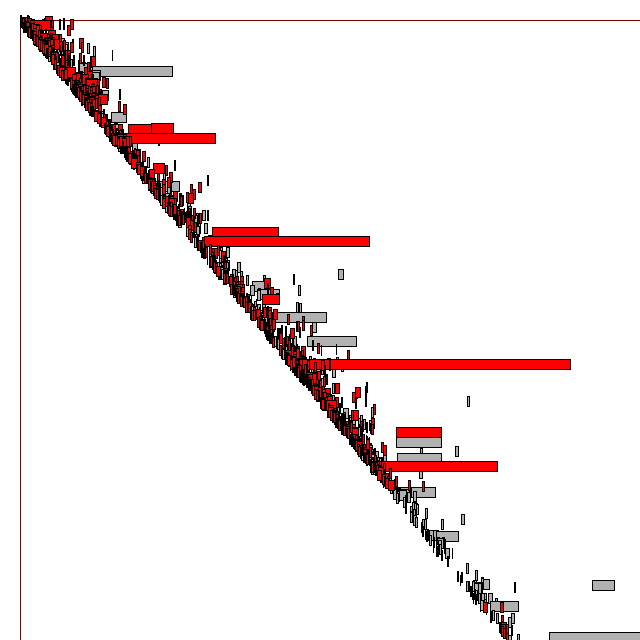
\includegraphics[width=0.45\linewidth]{figures/top_accepted.png}
}
\caption{\todo{for tobi: Explain.}}
\label{fig:timeline_view}
\end{figure}


\subsection{Prediction Model}
\begin{figure}[ht]
\centering
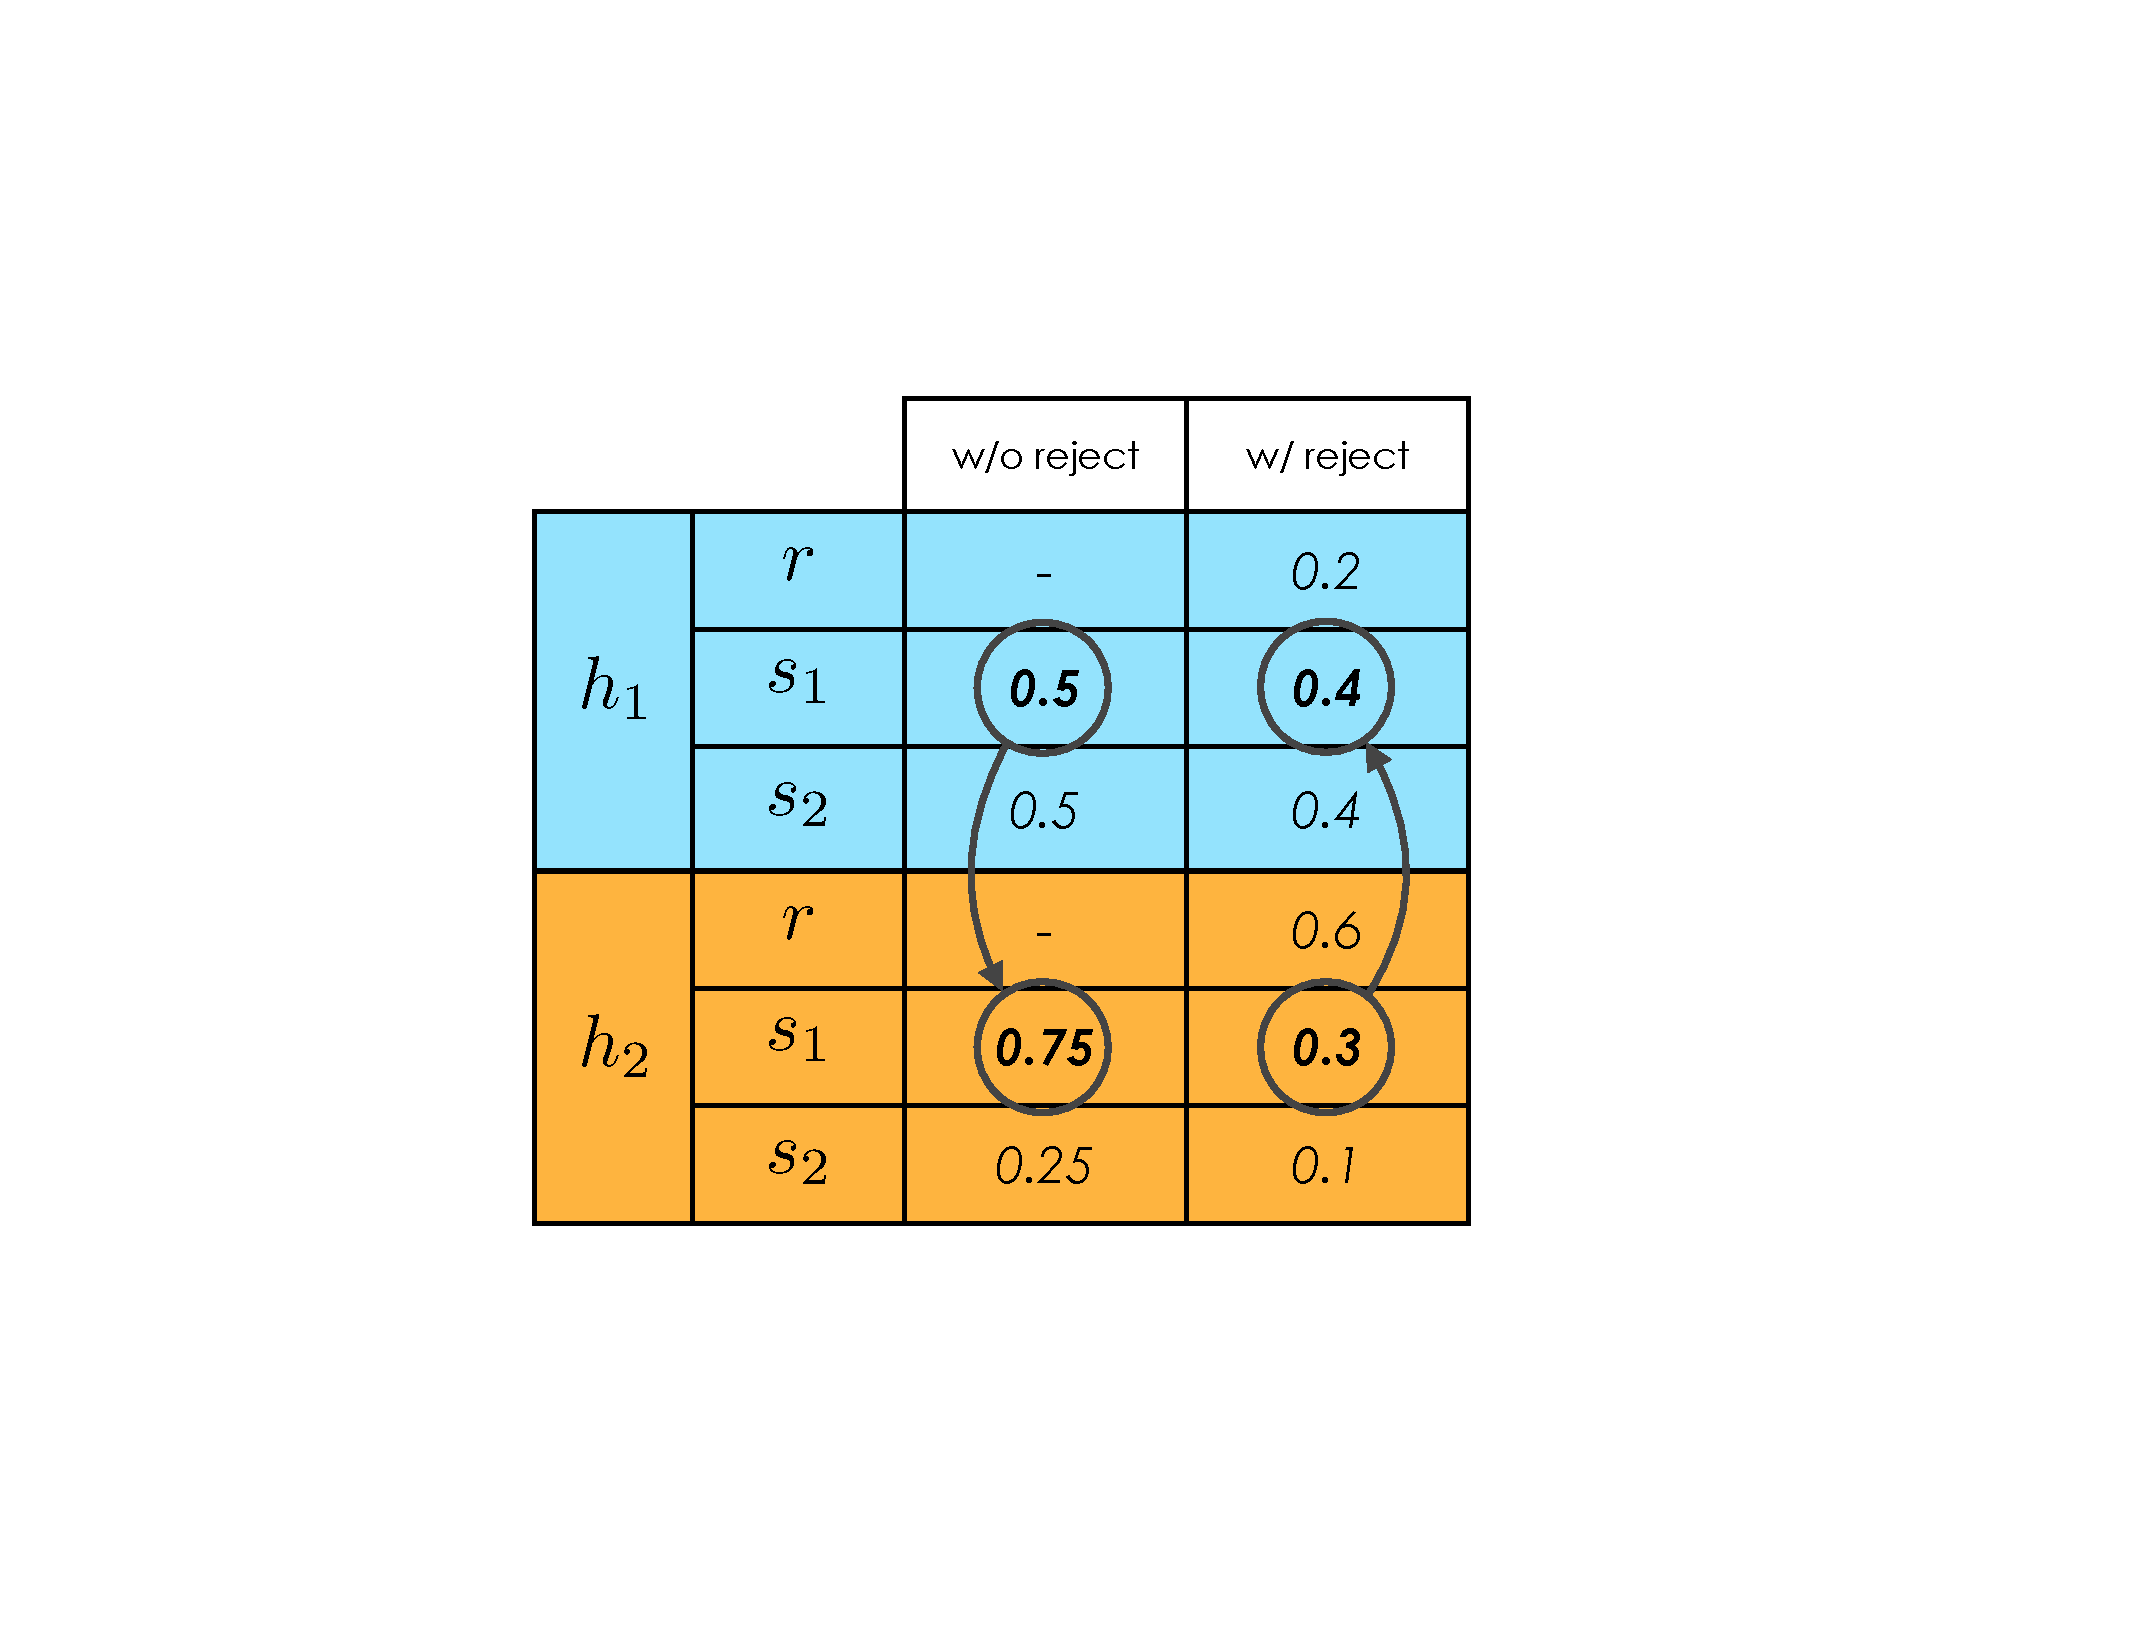
\includegraphics[width=0.6\linewidth]{figures/reject_vs_no_reject.pdf}
\caption{
Example of a case where modeling the reject option results in vastly different recommendation behavior.
Consider surfer $s_1$'s perspective: without modeling the reject option, $h_2$ looks more likely to accept $s_1$.
When modeling the reject option, however, the probabilities change and $h_1$ is now more likely to accept $s_1$, due to the ability to model how picky $h_2$ actually is.}
\label{fig:reject_vs_no_reject}
\end{figure}

We represent the probability that a host $h$ chooses surfer $s_k$ out of a competitor set $S$ with a logistic model
\begin{eqnarray}
p(s_k | h, S) &=& \frac{\exp(\theta^T \Phi(s_k,h,c)}{\sum_{s_j \in S} \exp(\theta^T \Phi(s_j,h,c)) + \exp(r)}
\end{eqnarray}
where $\Phi(s_k,h,c)$ is the output of the featurization function $\Phi: (s,h,c)  \mapsto \mathbb{R}^D$ and $\theta$ is the $D$-dimensional parameter vector we learn.
The parameter $c$ represents the context of the couch request, such as time, and will henceforth be omitted from notation but implictly included.
We also implictly model a bias term by appending $1$ to the representation $\Phi(s_k,h)$.

Accordingly, we model the probability that $h$ rejects all $s_k \in S$ as
\begin{eqnarray}
p(\text{reject} | h, S) &=& \frac{\exp(r)}{\sum_{s_j \in S} \exp(\theta^T \Phi(s_j,h)) + \exp(r)}
\end{eqnarray}

In this formulation, each surfer $s_k$ receives a score $\exp(\theta^T \Phi(s_k,h))$ modeling the natural competition between multiple surfers that requested to stay with the host.
In the end, we predict that the surfer with the highest score wins, or that everybody gets rejected if the ``reject score'' $\exp{(r)}$ is largest. 
Note, however, that this is not exactly the standard multinomial logistic regression model since in our case we have the same parameters but we have different features for the different ``classes'' (i.e. surfers). \todo{what does this mean?}

It may at first seem that we are essentially simply ranking the surfers, and so a reject option is not needed.
In fact, we are modeling the host decision process, and the reject option is very important.
As \autoref{fig:reject_vs_no_reject} demonstrates, the reject options enables us to model the ``pickiness'' of a host.
This allows us greater accuracy in predicting the decision outcomes for a competitor set, and allows CouchSurfing to rank potential hosts returned in a user search according to their actual likelihood of acceptance.

The parameters $\theta$ for this model should capture what hosts prefer in surfers and their request, i.e. their language, nationality, age, gender etc.
Because the feature $\Phi(s_k,h)$ depends on both the surfer and the host we also model that i.e. Americans like to host surfers from certain countries and that hosts generally prefer to have a language in common with the couchsurfer.
Further details are given in \autoref{sec:features}.

\subsubsection{Host preference personalization}
However, these preferences may be very different from host to host.
Also, some hosts might be more picky than others rejecting almost all requests and we should be able to capure that, too.
Therefore, we introduce host-specific parameters $\theta_h$ and $r_h$ to model these effects.
Because we have millions of hosts storing all these parameters explicitly would require tens of gigabytes of memory.

Since this is infeasible we make use of the ``hashing trick'' to hash the parameters into an array of predefined size (allowing for collisions between parameters).
Thereby, we can control how much memory we want to allocate for personalization.
This trick has been successfully applied e.g. for spam classification \cite{Attenberg2009}.

Including personalized parameters leads to the following updated model:
\begin{eqnarray}
p(s_k | h, S) &=& \frac{\exp((\theta + \theta_h)^T \Phi(s_k,h))}{\sum_{s_j \in S} \exp((\theta + \theta_h)^T \Phi(s_j,h)) + \exp(r + r_{h})} \\
p(\text{reject} | h, S) &=& \frac{\exp(r+r_{h})}{\sum_{s_j \in S} \exp((\theta + \theta_h)^T \Phi(s_j,h)) + \exp(r + r_{h})}
\end{eqnarray}

\subsubsection{Learning the parameters}
As an error measure, we use the negative log-likelihood of the data with $l_2$-penalty on the parameters for regularization.
In our Stochastic Gradient Descent (SGD), we randomly sample a host $h$ and a competitorset $S=\{ s_1, \dots, s_n\}$.
There are two cases: either there is one surfer $s_{k^*}$ that got accepted, or everybody got rejected.
We obtain the following update equations for SGD where $\lambda_1, \lambda_2$ are regularization parameters and $\eta$ is the learning rate

1. Case: Some surfer $s_{k^*}$ gets chosen.
\begin{eqnarray}
\theta &\leftarrow& (1- \eta \lambda_1) \theta - \eta (\sum_{j \in S_n} p(s_j | h, S) \Phi(s_j,h_n) - \Phi(s_{k^*},h_n))\\
r &\leftarrow& (1- \eta \lambda_2) r - \eta p(\text{reject} | h_n, S_n)
\end{eqnarray}

2. Case: No surfer gets chosen (reject).
\begin{eqnarray}
\theta &\leftarrow& (1- \eta \lambda_1) \theta - \eta (\sum_{j \in S_n} p(s_k | h, S) \Phi(s_j,h_n))\\
r &\leftarrow& (1- \eta \lambda_2) r - \eta (p(\text{reject} | h_n, S_n)-1)
\end{eqnarray}

The update equations for $\theta_h$ and $r_h$ are the same as the ones for $\theta$ and $r$, respectively, but they are only updated for the current host $h$.

These update equations make intuitive sense, as for $\theta$, we essentially increase the contribution from the features of the winner and decrease it for all the losers always according to their probability of being chosen.
This means that if the model did a bad prediction we update our parameters more than normally.
And for $r$, the story is similar in the sense that we increase the parameter value whenever everyone in the competitor set actually got rejected, and decrease it when we have a winner.

To scale the learning computation, we follow \cite{Zinkevich2010}'s SimuParallelSGD algorithm, and distribute random $T$-sized subsets of the data to $m$ different machines.
On each worker, SGD is used to update the parameters, sampling data in random order.
We modify the algorithm by repeating the above in a loop, each time averaging the per-machine parameter vectors and re-distributing them back to all workers.
The main idea of the algorithm is that in a large-scale learning situation such as concerns the CouchSurfing database, one can consider the present data to be a subset of a vritually infinite set, and so drawing with replacement and without replacement can both be simulated by shuffling the data and accessing it sequentially.

%%%%%%%%%%%%%%%%%%%%%%%%%%%
%-----------------OLD STUFF------
%\begin{eqnarray}
%p(s_k | h_n, S_n) &=& \frac{\exp(\theta^T \Phi(s_k,h_n))}{\sum_{j \in S_n} \exp(\theta^T \Phi(s_j,h_n)) + \exp(r + r_{h_n})} \\
%p(\text{reject} | h_n, S_n) &=& \frac{\exp(r+r_{h_n})}{\sum_{j \in S_n} \exp(\theta^T \Phi(s_j,h_n)) + \exp(r + r_{h_n})}
%\end{eqnarray}
%Note that $\Phi(s_k,h_n)$ also implicitly depends on the couchrequest (e.g. date, whether the host is already booked, etc.).
%
%To have hostspecific parameters we would replace $\theta$ by $\theta + \theta_h$. 
%
%Further, we want to add regularization for $\theta, \theta_h, r_{h_n}$.
%
%Error (negative log likelihood)
%\begin{eqnarray}
%E(\theta, r, r_{h_n}) &=& - \log p(\{s_k\} | \{h_n\}, \{S_n\})\\
%&=& - \log [ \prod_{n=1}^N \prod_{k=1}^K p(s_k | h_n, S_n)^{t_{nk}}]\\
%&=&  - \sum_{n=1}^N \sum_{k=1}^K t_{nk} \log p(s_k | h_n, S_n)
%\end{eqnarray}
%
%To derive the gradient descent update steps we will take derivatives of $E(\theta, r, r_{h_n})$ wrt. $\theta, r, r_{h_n}$. Because we will do stochastic gradient descent we will basically ignore the sum over $n$ in the end (over different ``competitor sets $S_n$'') and just choose one at random. Note that here, we can just sample uniformly from all sets or sample a host first, and given that host, sample on of his sets. The latter will achieve that all hosts have the sample influence on the learning but we will have to discuss/test whether we actually want that.
%
%We generally have:
%\begin{eqnarray}
%\frac{d}{d \theta} E(\theta, r, r_{h_n}) &=& - \sum_{n=1}^N \sum_{k=1}^K t_{nk} \frac{d}{d \theta}  \log p(s_k | h_n, S_n) \\
%&=& - \sum_{n=1}^N \sum_{k=1}^K t_{nk} \frac{1}{p(s_k | h_n, S_n)} \frac{d}{d \theta} p(s_k | h_n, S_n)
%\end{eqnarray}
%
%Now we look at the individual derivatives of $p(s_k | h_n, S_n)$ and $p(\text{reject} | h_n, S_n)$.
%
%1. Case: Some surfer $s_k$ gets chosen (no reject):
%\begin{eqnarray}
%\frac{d}{d \theta} p(s_k | h_n, S_n) = \frac{d}{d \theta} \frac{\exp(\theta^T \Phi(s_k,h_n))}{\sum_{j \in S_n} \exp(\theta^T \Phi(s_j,h_n)) + \exp(r + r_{h_n})} \\
%= \frac{\Phi(s_k,h_n) [\sum_{j \in S_n} \exp(\theta^T \Phi(s_j,h_n)) + \exp(r + r_{h_n})]}{\sum_{j \in S_n} \exp(\theta^T \Phi(s_j,h_n)) + \exp(r + r_{h_n})} \\
%- \frac{\exp(\theta^T \Phi(s_k,h_n)) [\sum_{j \in S_n} \Phi(s_j,h_n) \exp(\theta^T \Phi(s_j,h_n))]}{\sum_{j \in S_n} \exp(\theta^T \Phi(s_j,h_n)) + \exp(r + r_{h_n})}\\
%= \Phi(s_k,h_n) p(s_k | h_n, S_n) - p(s_k | h_n, S_n) \frac{\sum_{j \in S_n} \Phi(s_j,h_n) \exp(\theta^T \Phi(s_j,h_n))}{\sum_{j \in S_n} \exp(\theta^T \Phi(s_j,h_n)) + \exp(r + r_{h_n})}\\
%= p(s_k | h_n, S_n) (\Phi(s_k,h_n) - \sum_{j \in S_n} w_{jn} \Phi(s_j,h_n))
%\end{eqnarray}
%where $w_{jn}=\frac{\exp(\theta^T \Phi(s_j,h_n))}{\sum_{j \in S_n} \exp(\theta^T \Phi(s_j,h_n)) + \exp(r + r_{h_n})}$.
%
%Thus, we get:
%\begin{eqnarray}
%\frac{d}{d \theta} E(\theta, r, r_{h_n}) = - \sum_{n=1}^N \sum_{k=1}^K t_{nk} \frac{1}{p(s_k | h_n, S_n)} \frac{d}{d \theta} p(s_k | h_n, S_n)\\
%= - \sum_{n=1}^N \sum_{k=1}^K t_{nk} (\Phi(s_k,h_n) - \sum_{j \in S_n} w_{jn} \Phi(s_j,h_n)) \\
%= \sum_{n=1}^N (\sum_{j \in S_n} w_{jn} \Phi(s_j,h_n) - \Phi(s_{k^*},h_n))
%\end{eqnarray}
%where $s_{k^*}$ is the surfer that got accepted from the competitor set $S_n$.
%
%Similarly, taking the derivative wrt. $r$ ($r_{h_n}$ should be exactly the same) we obtain:
%\begin{eqnarray}
%\frac{d}{d r} p(s_k | h_n, S_n) = -  p(s_k | h_n, S_n)  \frac{\exp(r + r_{h_n})}{\sum_{j \in S_n} \exp(\theta^T \Phi(s_j,h_n)) + \exp(r + r_{h_n})}
%\end{eqnarray}
%Thus, we get:
%\begin{eqnarray}
%\frac{d}{d r} E(\theta, r, r_{h_n}) = - \sum_{n=1}^N \sum_{k=1}^K t_{nk} \frac{1}{p(s_k | h_n, S_n)} \frac{d}{d r} p(s_k | h_n, S_n)\\
%= \sum_{n=1}^N \sum_{k=1}^K t_{nk} \frac{\exp(r + r_{h_n})}{\sum_{j \in S_n} \exp(\theta^T \Phi(s_j,h_n)) + \exp(r + r_{h_n})} \\
%= \sum_{n=1}^N \frac{\exp(r + r_{h_n})}{\sum_{j \in S_n} \exp(\theta^T \Phi(s_j,h_n)) + \exp(r + r_{h_n})}
%\end{eqnarray}
%
%
%
%2. Case: No surfer gets chosen (reject):
%\begin{eqnarray}
%\frac{d}{d \theta} p(\text{reject} | h_n, S_n) = \frac{d}{d \theta} \frac{\exp(r+r_{h_n})}{\sum_{j \in S_n} \exp(\theta^T \Phi(s_j,h_n)) + \exp(r + r_{h_n})}\\
%= - p(\text{reject} | h_n, S_n) \frac{\sum_{j \in S_n} \Phi(s_j,h_n) \exp(\theta^T \Phi(s_j,h_n))}{\sum_{j \in S_n} \exp(\theta^T \Phi(s_j,h_n)) + \exp(r + r_{h_n})} \\
%= - p(\text{reject} | h_n, S_n) \sum_{j \in S_n} w_{jn} \Phi(s_j,h_n)
%\end{eqnarray}
%Thus, we get:
%\begin{eqnarray}
%\frac{d}{d \theta} E(\theta, r, r_{h_n}) = - \sum_{n=1}^N \sum_{k=1}^K t_{nk} \frac{1}{p(\text{reject} | h_n, S_n)} \frac{d}{d \theta} p(\text{reject} | h_n, S_n)\\
%= \sum_{n=1}^N (\sum_{j \in S_n} w_{jn} \Phi(s_j,h_n))
%\end{eqnarray}
%
%
%
%Again, taking the derivative wrt. $r$ ($r_{h_n}$ should be exactly the same) we obtain:
%\begin{eqnarray}
%\frac{d}{d r} p(\text{reject} | h_n, S_n) = p(\text{reject} | h_n, S_n) - p(\text{reject} | h_n, S_n)^2\\
%= p(\text{reject} | h_n, S_n) (1 - p(\text{reject} | h_n, S_n))\\
%\end{eqnarray}
%Thus, we get:
%\begin{eqnarray}
%\frac{d}{d r} E(\theta, r, r_{h_n}) = - \sum_{n=1}^N \sum_{k=1}^K t_{nk} \frac{1}{p(\text{reject} | h_n, S_n)} \frac{d}{d \theta} p(\text{reject} | h_n, S_n)\\
%= \sum_{n=1}^N (p(\text{reject} | h_n, S_n)-1)
%\end{eqnarray}
%
%
%\paragraph{The final update equations}
%
%Finally, for stochastic gradient descent the following update equations hold. We simply sample a host $h_n$ and competitor set $S_n$. Note that the following equations do not contain regularization, yet (although trivial).
%
%1. Case: Some surfer $s_{k^*}$ gets chosen (no reject):
%\begin{eqnarray}
%\theta \leftarrow \theta - \eta (\sum_{j \in S_n} w_{jn} \Phi(s_j,h_n) - \Phi(s_{k^*},h_n))\\
%r \leftarrow r - \eta \frac{\exp(r + r_{h_n})}{\sum_{j \in S_n} \exp(\theta^T \Phi(s_j,h_n)) + \exp(r + r_{h_n})}
%\end{eqnarray}
%where, again, $w_{jn}=\frac{\exp(\theta^T \Phi(s_j,h_n))}{\sum_{j \in S_n} \exp(\theta^T \Phi(s_j,h_n)) + \exp(r + r_{h_n})}$.
%
%2. Case: No surfer gets chosen (reject):
%\begin{eqnarray}
%\theta \leftarrow \theta - \eta (\sum_{j \in S_n} w_{jn} \Phi(s_j,h_n))\\
%r \leftarrow r - \eta (p(\text{reject} | h_n, S_n)-1)
%\end{eqnarray}
%
%For $l_2$-regularization, e.g. of $\theta$, just add $- \eta \lambda \theta$ to the update equation.
%
